\documentclass[a4paper,10pt]{article}
\usepackage{amsmath,amssymb,graphicx,float,subfig}

%defines
\def\bY{{\bf Y}}
\def\bX{{\bf X}}
\def\bE{{\bf E}}
\def\bV{{\bf V}}
\def\bC{{\bf C}}
\def\bH{{\bf H}}
\def\b1{{\bf 1}}
\def\bx{{\bf x}}
\def\bs{{\bf s}}
\def\bh{{\bf h}}
\def\blambda{{\boldsymbol \lambda}}
\def\bgamma{{\boldsymbol \gamma}}
\def\bbeta{{\boldsymbol \beta}}
\def\btheta{{\boldsymbol \theta}}
\def\bnu{{\boldsymbol \nu}}
\def\bmu{{\boldsymbol \mu}}
\def\sigmaeps{{\sigma_{\epsilon}}}

%opening
\title{Home Assignment - 1}
\author{Santhosh Nadig, Zhanzhang Cai}

\begin{document}

\maketitle

\section{Introduction}
Spatially consecutive temperature data is an important evaluating criterion of global/regional climate model and a pivotal driver of dynamic vegetation model. In spatial statistics, a common situation is to reconstruct (interpolate) values at unobserved locations from observations at some measurement locations. In this assignment, we will reconstruct average monthly temperature for Sweden during June of 2005, using observations from weather stations. Ordinary least squares and universal Kriging will be tested for their performance in reconstructing the monthly average temperature at the validation sites and on the prediction grid.
\section{Theory}
Let $\bY_k$ represent the $n$ known observations of spatial data and $\bY_u$ represent the $m$ data points that needs to be estimated. For ordinary Kriging ($\mu = \b1 \beta$), the optimal predictions are given by
\begin{align*}
 \hat \bY_u &= \b1_u \hat \beta + \Sigma_{uk} \Sigma_{kk}^{-1}\left( \bY_k - \b1_k \hat \beta \right) \\
 \hat \beta &= \left( \b1_k^T \Sigma_{kk}^{-1} \b1_k \right)^{-1} \b1_k^T \Sigma_{kk}^{-1} \bY_k,
\end{align*}
where
\begin{align*}
 &\begin{bmatrix}
  \bY_k \\
  \bY_u
 \end{bmatrix} \in
 \mathbf{N} \left( 
 \begin{bmatrix}
    \b1_k \beta \\
   \b1_u \beta
  \end{bmatrix},
  \begin{bmatrix}
   \Sigma_{kk} & \Sigma_{ku} \\
   \Sigma_{uk} & \Sigma_{uu}
  \end{bmatrix}
  \right).
\end{align*}

Firstly, we show that the predictions are linear in the observations, i.e., $\hat \bY_u = \blambda^T \bY_k$ for some $\blambda$. We may re-write $\hat \beta$ as
\begin{align*}
 \hat \beta &= \bgamma^T \bY_k \\
 \bgamma &= \left( \left( \b1_k^T \Sigma_{kk}^{-1} \b1_k \right)^{-1} \b1_k^T \Sigma_{kk}^{-1} \right)^T.
\end{align*}
We note that the vector $\bgamma^T$ is of dimensions $1 \times n$, and therefore, $\hat \beta$ is a scalar. Substituting the above in the expression for $\hat \bY_u$, we obtain
\begin{align*}
 \hat \bY_u &= \b1_u \bgamma^T \bY_k + \Sigma_{uk} \Sigma_{kk}^{-1} \bY_k -  \Sigma_{uk} \Sigma_{kk}^{-1}  \b1_k \bgamma^T \bY_k \\
      &= \left( \b1_u \bgamma^T + \Sigma_{uk} \Sigma_{kk}^{-1} -  \Sigma_{uk} \Sigma_{kk}^{-1}  \b1_k \bgamma^T \right) \bY_k \\
      &= \blambda^T \bY_k,
\end{align*}
where $\blambda = \left( \b1_u \bgamma^T + \Sigma_{uk} \Sigma_{kk}^{-1} -  \Sigma_{uk} \Sigma_{kk}^{-1}  \b1_k \bgamma^T \right)^T$.

Secondly, we show that the predictions are unbiased, i.e., $\bE(\hat \bY_u) = \bE(\bY_u)$. The expected value of $\hat \beta$ is given by
\begin{align*}
 \bE \left( \hat \beta \right) &= \left( \b1_k^T \Sigma_{kk}^{-1} \b1_k \right)^{-1} \b1_k^T \Sigma_{kk}^{-1} ~ \bE (\bY_k) \\
  &= \left( \b1_k^T \Sigma_{kk}^{-1} \b1_k \right)^{-1} \b1_k^T \Sigma_{kk}^{-1} ~ \b1_k \beta \\
  &= \beta.
\end{align*}
Therefore,
\begin{align*}
 \bE(\hat \bY_u) &=  \b1_u \bE\left(\hat \beta \right) + \Sigma_{uk} \Sigma_{kk}^{-1}\left( \bE(\bY_k) - \b1_k \bE \left(\hat \beta \right)\right) \\
 &= \b1_u \beta + \Sigma_{uk} \Sigma_{kk}^{-1}\left( \b1_k \beta - \b1_k \beta \right) \\
 &= \b1_u \beta.
\end{align*}

Finally, consider a second unbiased predictor of $\bY_u$, given by $\tilde \bY_u = (\blambda + \bnu)^T \bY_k$. From the unbiasedness criterion, we have that $\bE(\tilde \bY_u) = \bE(\hat \bY_u)$. Therefore, $(\blambda + \bnu)^T \bE(\bY_k) = \blambda^T \bE(\bY_k)$, implying $\bnu^T \b1_k = 0$. Furthermore, consider the variance of the second predictor
\begin{align*}
 \bV(\tilde \bY_u - \bY_u) &= \bV(\bnu^T \bY_k + (\blambda^T \bY_k - \bY_u))\\
 &= \bV(\bnu^T \bY_k) + \bV(\hat \bY_u - \bY_u) + 2\bC(\bnu^T \bY_k, \hat \bY_u - \bY_u) \\
 &\ge \bV(\hat \bY_u - \bY_u) + 2\bC(\bnu^T \bY_k, \hat \bY_u - \bY_u)\\
 &= \bV(\hat \bY_u - \bY_u) + 2\bnu^T \bC(\bY_k, \hat \bY_u) - 2 \bnu^T \bC(\bY_k, \bY_u) \\
 &= \bV(\hat \bY_u - \bY_u) + 2\bnu^T \left(  \Sigma_{kk} \blambda - \Sigma_{uk}\right)
\end{align*}
Thus, if we can choose $\blambda$ such that $\bnu^T \left(  \Sigma_{kk} \blambda - \Sigma_{uk}\right) = 0$, then, we have that $\bV(\tilde \bY_u - \bY_u) \ge \bV(\hat \bY_u - \bY_u)$ for any unbiased predictor $\tilde \bY_u$.

\section{Swedish Temparature Reconstruction}
The dataset ({\texttt{SweObs}}) consists of average temperature during June 2005 measured at 250 stations across Sweden. The corresponding latitude, longitude, elevation and distance to both the Swedish coast and to any coastline are provided too. Figure \ref{fig:rawdataplot} shows the plot of average temperature, elevation and distance to any coast. The average temperatures are higher in the South (lower latitudes) and towards the coast, as expected. The \texttt{SweGrid} consists of a grid of 273-by-260 locations at which the average temperature should be predicted. We examine two methods -- ordinary least squares (OLS) and Kriging in the forthcoming sections.
\begin{figure}[ht]
	\centering
	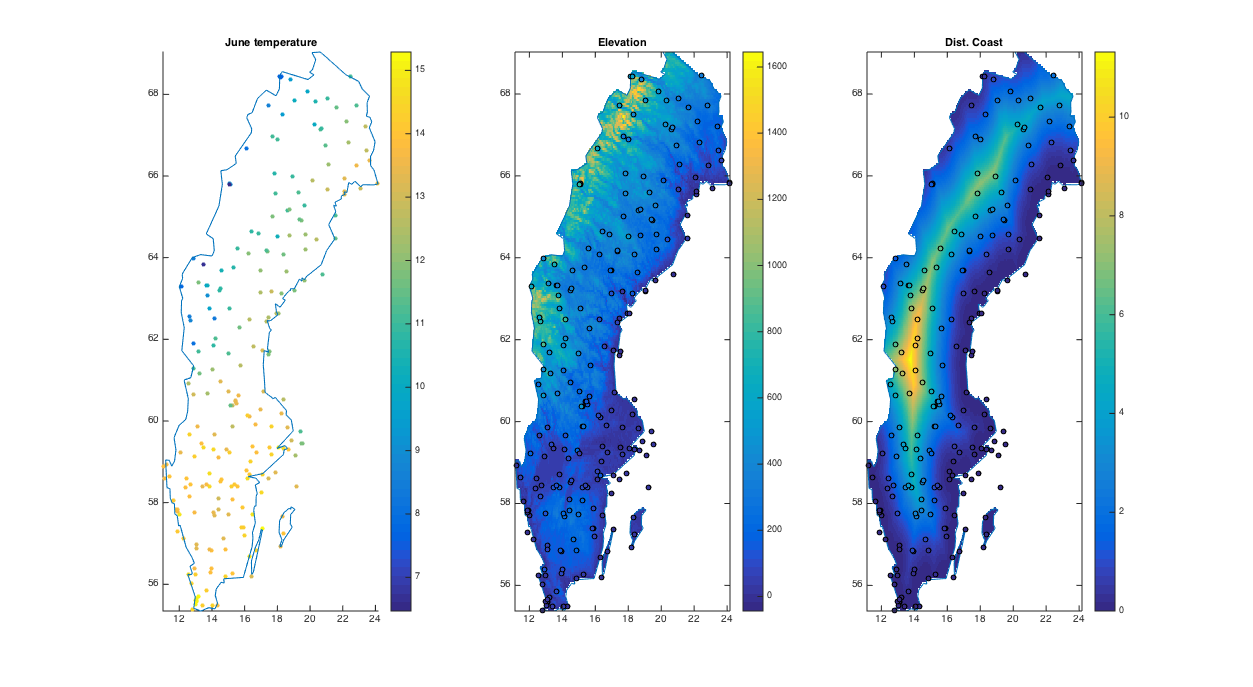
\includegraphics[width=0.8\linewidth]{raw_data_plot.png}
	\caption{Plots showing (R-L) average temperature in June 2005, elevation and distance to any coastline.}
	\label{fig:rawdataplot}
\end{figure}
\subsection{Ordinary Least Squares}
The average temperature (observations), $\bY$ is modelled as a linear function of the covariates. 
\begin{equation*}
  \bY \triangleq \bX \bbeta +  {\boldsymbol \epsilon} 
\end{equation*}
where $\bX$ is the covariate matrix, $\bbeta$ is the parameter vector and ${\boldsymbol \epsilon} \in N(0, \sigmaeps^2 \mathbb{I})$.

Figure \ref{fig:covariates} shows a plot of the observations as a function of the available covariates from {\texttt{SweObs}}.
\begin{figure}[ht]
	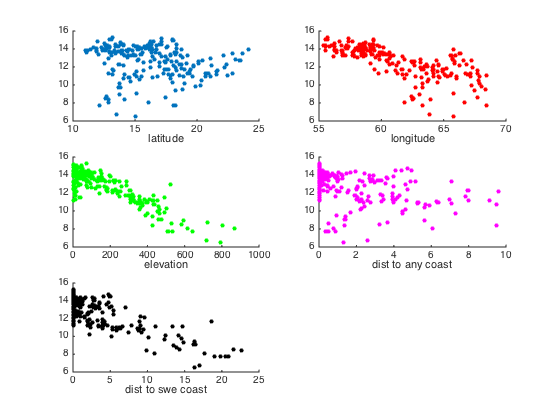
\includegraphics[width=0.8\linewidth]{covariates.png}
	\caption{Observation vs covariates}
	\label{fig:covariates}
\end{figure}
It was found that longitude does not relate linearly with the average temperatures measured and hence is left out of modelling. In order to select the appropriate covariates, we formed five models (A,B,C,D,E) containing different set of covariates as tabulated in Table \ref{tab:models}.
\begin{table}[H]
\centering
\begin{tabular}{lp{9cm}}
\hline
{\bf Model} & {\bf Covariates} \\
\hline
* A & Latitude, elevation, distance to any coast, distance to Swedish coast\\
 B & Latitude, elevation, distance to Swedish coast\\
 C & Latitude, elevation, distance to any coast\\
 D & Latitude, distance to any coast, distance to Swedish coast\\
 E & Latitude, elevation\\
\hline
\end{tabular}
\caption{Models and the respective covariates, with average temperature as the independent varible.}
\label{tab:models}
\end{table}
The standard errors of the residuals and the Akaike Information Criterion (AIC) seen in figure \ref{fig:modperf} shows that model A performs best.
\begin{figure}[ht]
\centering
  \subfloat[Std. Err of the residuals for each of the models.]{{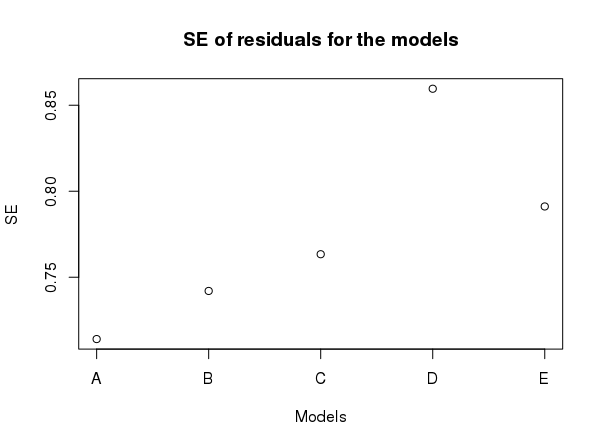
\includegraphics[width=5cm]{RSS_models.png} }}%
  \qquad
  \subfloat[AIC for each of the models.]{{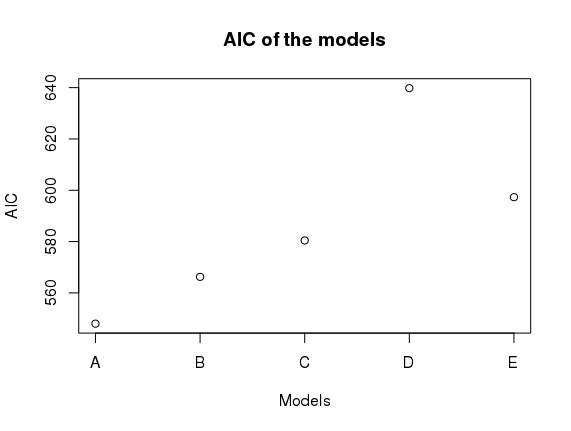
\includegraphics[width=5cm]{AIC_models.png} }}%
  \caption{Performance evaluation of the five models (A,B,C,D,E). Model A has the least Std. Err of the residuals and the best AIC metric.}
\label{fig:modperf}
\end{figure}

Thus, using model A, we may express the observations $\bY$ as a linear function of latitude ($\bx_1$), elevation ($\bx_2$), distance to any coast ($\bx_3$) and the distance to Swedish coast ($\bx_4$).
\begin{equation}
 \bY = \beta_0 + \beta_1 \bx_1 + \beta_2 \bx_2 + \beta_3 \bx_3 + + \beta_4 \bx_4 + {\boldsymbol \epsilon}
\end{equation}
where $\beta_0 \dots \beta_4$ are the parameters. For  validation, 25 randomly picked observations are set aside and we use $N = 225$ data points for the model parameter estimation. The estimated parameters and variance are given by
\begin{align*}
& \hat \bbeta = (\bX^T \bX)^{-1} \bX^T \bY\\
& \bV(\hat \bbeta | \sigmaeps^2) = \sigmaeps^2 (\bX^T \bX)^{-1}
\end{align*}
 The estimated parameters (and their standard errors ) are tabulated below.
\begin{table}[H]
\centering
\begin{tabular}{lcc}
\hline
{\bf Parameter} & {\bf Estimate} & {\bf SE }\\
\hline
$\hat \beta_0$ & 23.972 & 0.95 \\
$\hat \beta_1$ & -0.169 & 0.016\\
$\hat \beta_2$ & -0.005 & 0.0005 \\
$\hat \beta_3$ & 0.106 & 0.025\\
$\hat \beta_4$ & -0.089 & 0.015\\
\hline
\end{tabular}
\caption{Parameter Estimates and corresponding standard errors (OLS).}
\label{tab:olsest}
\end{table}
The variance of the residuals $\sigmaeps^2 = 0.48$. The mean temperatures at the validation points are given by
\begin{equation}
\bE(\hat \bY_v) = \bX_v \hat \bbeta
\end{equation}
where $\hat \bY_v$ denotes the average temperature estimates at the validation points, $\bX_v$  the regressor matrix formed using the latitude, elevation, distance to any coast and distance to Swedish coast of the 25 validation points and $\hat \bbeta$ the estimated model parameters. The variance and the 95\% confidence interval are given by
\begin{align*}
\bV(\hat \bY_v) &= \sigmaeps^2 (\bX_v (\bX_v^T\bX_v)^{-1} \bX_v^T + 1) \\
\text{CI, 95\%} &= \bE(\hat \bY_v) \pm 1.96 \text{ SE}(\hat \bY_v)
\end{align*}
where $\text{SE}(\hat \bY_v) = \sqrt{\bV(\hat \bY_v)}$. Figure \ref{fig:olsglsval}(a) shows a plot of prediction and confidence intervals for the validation points. The predictions for the {\texttt{SweGrid}} data along with the corresponding standard error are shown in figure \ref{fig:olsresults}.
\begin{figure}[ht]
\centering
  \subfloat[]{{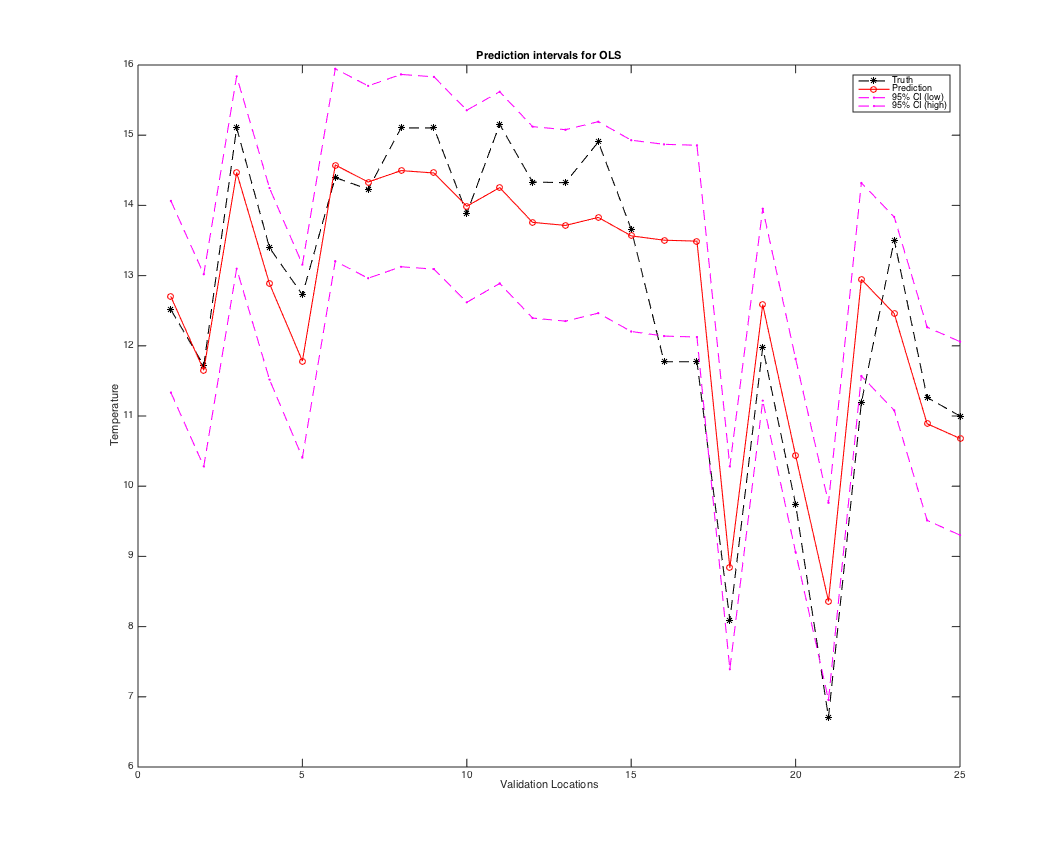
\includegraphics[width=4.8cm]{ols_valdat_pred_ci.png} }}%
  \qquad
  \subfloat[]{{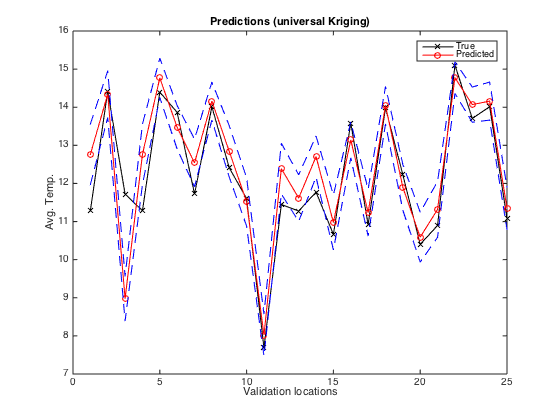
\includegraphics[width=5cm]{krig_val_pred.png} }}%
  \caption{(a): Estimate and confidence intervals (95\%) for the 25 validation points with OLS estimate. (b) Estimate and confidence intervals (95\%) for the 25 validation points with GLS estimate.}
\label{fig:olsglsval}
\end{figure}

\subsection{Universal Kriging}
Firstly, we proceed to evaluate the spatial dependence in the residuals from the OLS model. A non-parametric approach (binned covariance function estimation [slide 13 lecture 03]) with 33 bins is used for this purpose. Figure \ref{fig:covnp}(a) shows the estimated covariance function of the residuals (as a function of the bins), where the bin $\bH_k = \{ (i,j): i \ne j, kh \le \| \bs_j - \bs_i \| < (k+1)h \}$. The confidence intervals are generated by the boxplot where the first and the third quantiles (25, 75) are shown. Thus, we see that there is a trend where the spatial dependence decreases with distance (at least, to some point). We also note that the covariance function estimate for large distances tend to be biased due to fewer samples in those bins as shown in figure  \ref{fig:covnp}(b).
\begin{figure}[ht]
\centering
  \subfloat[Binned covariance function with quantiles.]{{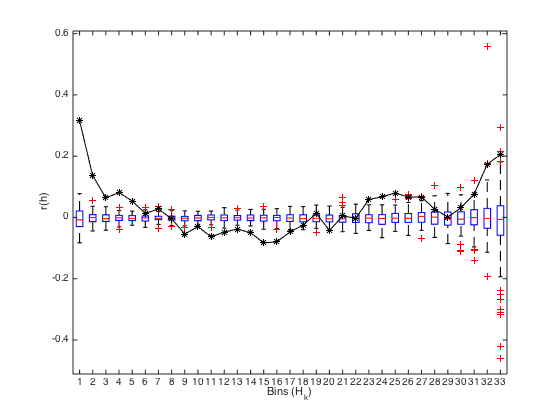
\includegraphics[width=5cm]{binned_covfun.png} }}%
  \qquad
  \subfloat[Number of observations per bin]{{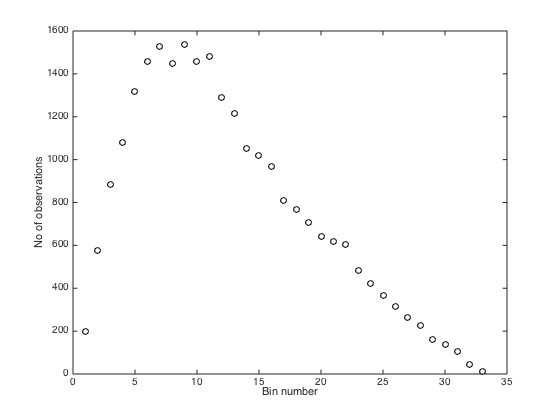
\includegraphics[width=5cm]{num_obs_per_bin.png} }}%
  \caption{Estimated Covariance function (non-parametric) with $K = 33$ bins and the number of observations in each bin.}
\label{fig:covnp}
\end{figure}
Secondly, a parametric model is chosen to fit the empirical covariance function (determined using the binning method as mentioned above). The chosen model is the Matern covariance function $r_M(\bh)$ [slide 4, lecture 3] given by  
\begin{equation*}
r_M(\bh) = \frac{\sigma^2}{\Gamma(\nu) 2^{(\nu - 1)}} (\kappa \| \bh \|)^{\nu} K_{\nu}(\kappa \| \bh \|)^{\nu}, \qquad \bh \in \mathbb{R}^d,
\end{equation*}
whose parameters $\btheta = [\kappa, \sigma^2, \nu]$ are estimated using the least squares method.
\begin{equation*}
\hat \theta = \arg \min_{\btheta} \sum_{i=1}^n (y_i - \bE(y_i; \theta)).
\end{equation*}

Since we now have an estimate of the covariance matrix (from the parametric model), we use the Generalized Least Squares (GLS) to compute a refined estimate of $\bbeta$. The GLS estimate of $\bbeta$ and the corresponding variance is given by
\begin{align*}
& \hat \bbeta = (\bX^T \Sigma^{-1} \bX)^{-1} \bX^T \Sigma^{-1} \bY \\
& \bV(\bbeta | \sigmaeps^2, \Sigma) = \sigmaeps^2 (\bX^T \Sigma^{-1} \bX)^{-1}
\end{align*}

With the new estimate of $\bbeta$, we form another set of residuals with which we iterate the above procedure 3 times (the steps are as described in slide 16 of lecture 3). The parameter estimates and the corresponding standard errors are tabulated in Table \ref{tab:glsest}.
\begin{table}[ht]
\centering
\begin{tabular}{lcc}
\hline
{\bf Parameter} & {\bf Estimate} & {\bf SE }\\
\hline
$\hat \beta_0$ & 20.2 & 3.75 \\
$\hat \beta_1$ & -0.108 & 0.001\\
$\hat \beta_2$ & -0.005 & 1.7e-7 \\
$\hat \beta_3$ & 0.102 & 0.001\\
$\hat \beta_4$ & -0.11 & 0.003\\
\hline
\end{tabular}
\caption{Parameter Estimates and corresponding standard errors (GLS).}
\label{tab:glsest}
\end{table}

Finally, the Kriging estimator for predicting the temperatures at the `unknown' locations ($\bY_u$) and the corresponding variance (adjusting for the estimated $\bbeta$s) is given by
\begin{gather*}
\bY_u = \bX_u \bbeta + \Sigma_{uk} \Sigma_{kk}^{-1} (\bY_k - \bX_k \bbeta) \\
\begin{split}
\bV(y_u| \bY_k, \btheta, \hat \bbeta) &= \Sigma_{uu} -  \Sigma_{uk} \Sigma_{kk}^{-1}\Sigma_{ku} + \\
&(\bX_u^T - \bX_k^T \Sigma_{kk}^{-1}\Sigma_{ku})^T ( \bX_k^T \Sigma_{kk}^{-1} \bX_k)^{-1} (\bX_u^T - \bX_k^T \Sigma_{kk}^{-1}\Sigma_{ku})
\end{split}
\end{gather*}

The estimated model parameters are validated using the 25 randomly chosen validation locations. Figure shows a plot of the true and predicted temperatures together with the confidence intervals for the validation locations. A plot of the prediction and standard errors for the predictions of the {\texttt{SweGrid}} data is shown in figure \ref{fig:krigresults}. It is apparent that the predictions from Kriging method has lower variance compared to those from the OLS method.

\begin{figure}[ht]
\centering
  \subfloat[Estimate of average temperature]{{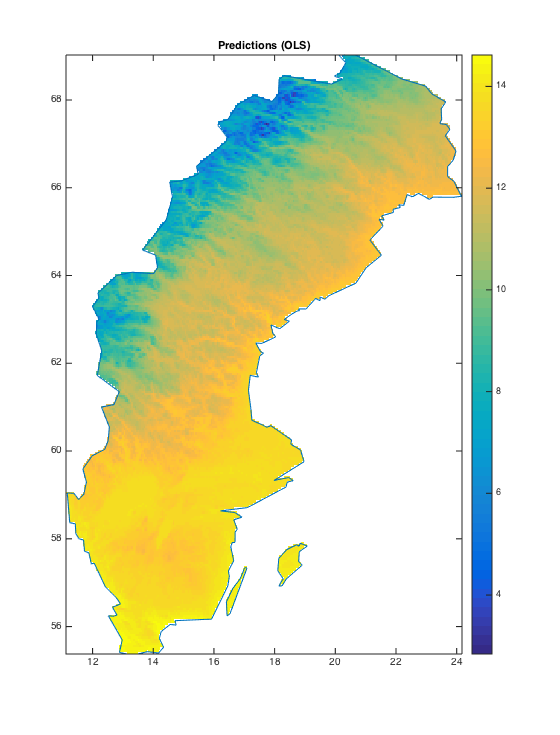
\includegraphics[width=5cm,height=7cm]{pred_ols_grid.png} }}%
  \qquad
  \subfloat[Standard Error]{{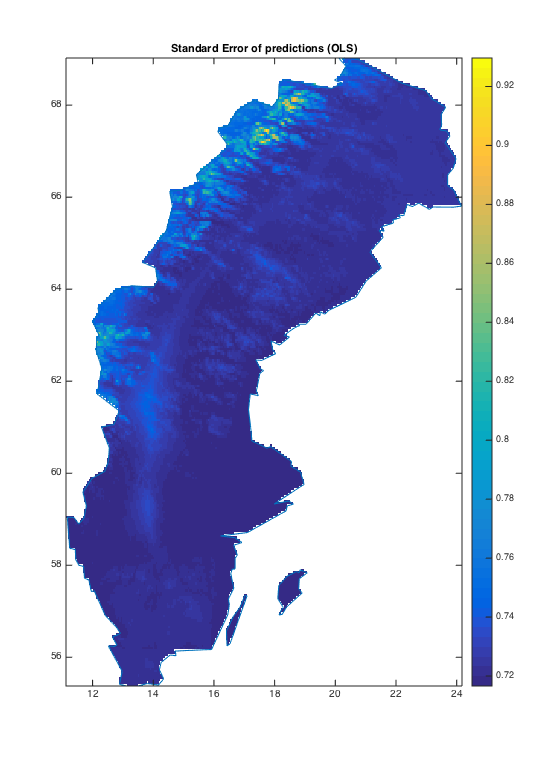
\includegraphics[width=5cm,height=7cm]{se_pred_ols.png} }}%
  \caption{OLS estimates and standard error for \texttt{SweGrid} locations.}
\label{fig:olsresults}
\end{figure}
\begin{figure}[H]
\centering
  \subfloat[Estimate of average temperature]{{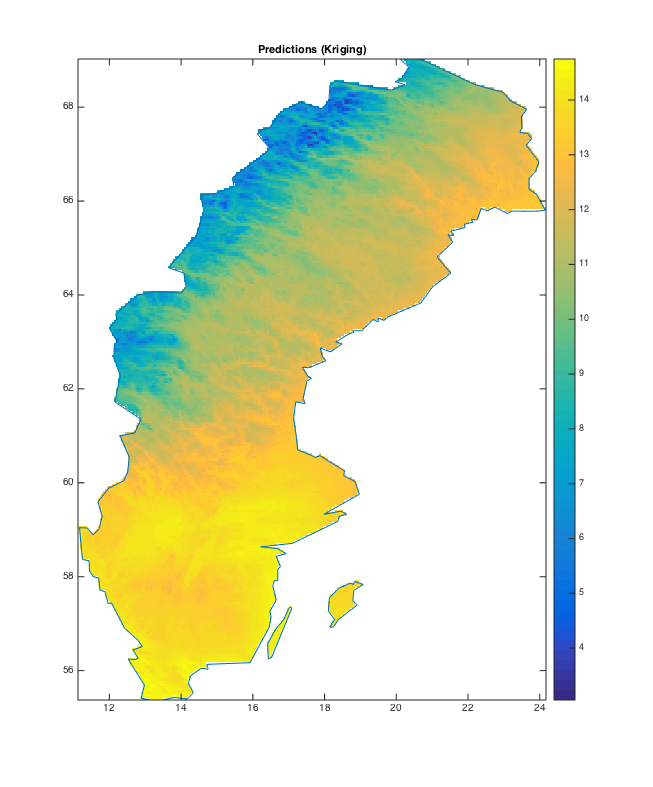
\includegraphics[width=5cm,height=7cm]{pred_krig_grid.png} }}%
  \qquad
  \subfloat[Standard Error]{{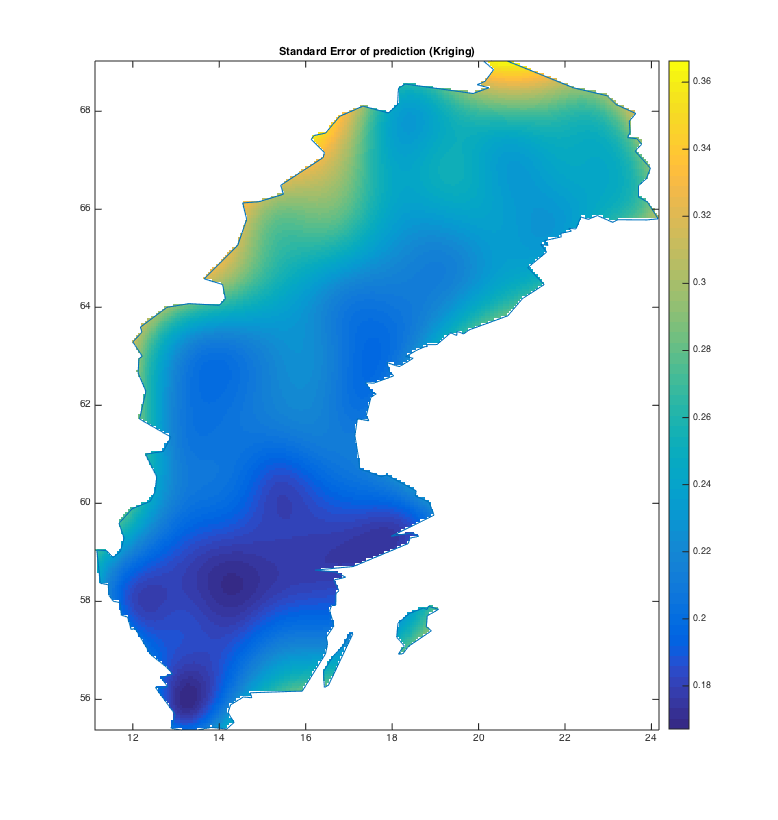
\includegraphics[width=5cm,height=7cm]{se_pred_krig.png} }}%
  \caption{Krigining estimates and standard error for \texttt{SweGrid} locations.}
\label{fig:krigresults}
\end{figure}

\section{Conclusions}
In this report we examined two estimation methods, ordinary least squares and Krigining, for estimating the spatial process of the average temperature in June 2005 at various locations in Sweden. The ordinary least squares method is attractive due to its simplicity. However, the variance of the estimated model parameters and predictions is higher compared to that from Kriging method. Additionally, OLS may suffer in the presence of outliers and/or missing data in a region unless some care is taken (like outlier analysis and ensuring that known observations are spatially spread, etc.)

\end{document}
